\documentclass[preprint,12pt]{elsarticle}

\usepackage{amssymb}
\usepackage{amsmath}
\usepackage{amsthm}
\usepackage[utf8]{inputenc}
\usepackage{graphicx}
\usepackage{xurl}
\usepackage[hidelinks]{hyperref}

\journal{Discrete Mathematics}

\newcommand{\zenodoID}{10.5281/zenodo.0000000}
\newcommand{\preprintURL}{https://github.com/creelie/urban-chainsaw/blob/main/preprintKourovka2071b/Kourovka2071b.pdf}

\newtheorem{theorem}{Theorem}[section]
\newtheorem{proposition}[theorem]{Proposition}
\newtheorem{lemma}[theorem]{Lemma}
\newtheorem{corollary}[theorem]{Corollary}
\theoremstyle{definition}
\newtheorem{definition}[theorem]{Definition}
\newtheorem{remark}[theorem]{Remark}

\newcommand{\F}{\mathbb{F}}
\newcommand{\Tr}{\operatorname{Tr}}
\newcommand{\Aut}{\operatorname{Aut}}

\begin{document}

\begin{frontmatter}

\title{A graph with three card types and five vertex orbits}

\author[egspl]{Deep Bhattacharjee\corref{cor1}\fnref{orcid1}}
\ead{itsdeep@live.com}
\ead{d.bhattacharjee@erl-forschung.de}
\fntext[orcid1]{ORCID: \url{https://orcid.org/0000-0003-0466-750X}}
\cortext[cor1]{Corresponding author.}
\affiliation[egspl]{organization={Formerly, Electro-Gravitational Space Propulsion Laboratory (EGSPL)},
            city={Bhubaneswar},
            postcode={751030},
            state={Odisha},
            country={India}}

\author[ntu]{Ushashi Bhattacharya\fnref{orcid2}}
\ead{rai.bhattacharya.in@gmail.com}
\fntext[orcid2]{ORCID: \url{https://orcid.org/0009-0002-2254-3914}}
\affiliation[ntu]{organization={Formerly, National Taiwan University},
            city={Taipei},
            postcode={106319},
            country={Taiwan}}

\begin{abstract}
We prove that the answer to part~(b) of Problem~20.71 of the Kourovka Notebook is yes: there is a connected graph on $63$ vertices with exactly three isomorphism types of vertex-deleted subgraphs whose automorphism group has five orbits on the vertices. The graph is a Cayley graph of a Suzuki $2$-group of order $64$ with one vertex removed.
\end{abstract}

\begin{keyword}
vertex-deleted subgraph \sep pseudosimilar vertices \sep Cayley graph \sep Suzuki $2$-group \sep divisible design graph
\MSC[2020] Primary 05C60 \sep Secondary 05C25 \sep 20D15 \sep 68V15
\end{keyword}

\end{frontmatter}

\section{Introduction}\label{sec:intro}

All graphs are finite and simple. For a vertex $v$ of a graph $G$, the \emph{card} $G-v$ is the subgraph induced on $V(G)\setminus\{v\}$. Let $k(G)$ be the number of isomorphism classes of cards of $G$ and $r(G)$ the number of orbits of $\Aut(G)$ on $V(G)$. An automorphism mapping $u$ to $v$ restricts to an isomorphism $G-u\to G-v$, so $k(G)\le r(G)$. Vertices $u,v$ in different orbits with $G-u\cong G-v$ are called \emph{pseudosimilar}; they exist exactly when $k(G)<r(G)$.

Problem~20.71 of the Kourovka Notebook \cite{Kourovka}, posed by J.~Lauri and communicated by V.~Pannone, reads: ``For a connected graph $G$ with $k$ isomorphism types of cards, can $\Aut(G)$ have more than $k$ orbits on the vertex set $V(G)$ a) for $k=2$? b) for $k=3$? c) for $k=4$?'' The comment to the problem records that $r(G)=1$ when $k(G)=1$, and that connected graphs with $(k,r)=(5,6)$ and $(6,7)$ are known. Prajapati \cite{Prajapati} answered (c) with a connected graph on $9$ vertices having $k=4$ and $r=5$, and found by exhaustive search that no connected graph on at most $12$ vertices answers (a) or (b). We answer (b).

\begin{theorem}\label{thm:main}
There is a connected graph $X$ on $63$ vertices with $k(X)=3$ and $r(X)=5$.
\end{theorem}

The graph $X$ is obtained from a Cayley graph $Y$ of a Suzuki $2$-group $H$ of order $64$ \cite{Higman} by deleting the identity. Left multiplications of $H$ make $X-x$ isomorphic to $X-x^{-1}$, and inversion of $H$ exchanges two pairs of $\Aut(X)$-orbits (Section~\ref{sec:cards}). The proof that these orbits are distinct rests on the fact that $Y$ is a divisible design graph \cite{HKM}: two distinct vertices have two common neighbours if they lie in the same coset of the centre of $H$ and three otherwise (Section~\ref{sec:graph}). The cosets carry a Fano plane defined by the graph, which separates the orbits (Section~\ref{sec:orbits}). The whole proof is formalized in Lean~4 and checked by its kernel (Section~\ref{sec:lean}). Part~(a) remains open.

\section{The group and the graph}\label{sec:graph}

Let $\F=\F_2[t]/(t^3+t+1)$ be the field with $8$ elements and $\F^\times=\F\setminus\{0\}$. Cubing is a bijection of $\F^\times$, since $\gcd(3,7)=1$. Let $\Tr(\beta)=\beta+\beta^2+\beta^4$ be the trace to $\F_2$, so $\Tr(1)=1$. Put
\[
R_0=\{t,t^2,t^4\},\qquad R_1=\{t+1,t^2+1,t^4+1\},
\]
the roots of $x^3+x+1$ and of $x^3+x^2+1$; then $\F=\{0,1\}\cup R_0\cup R_1$, $\Tr$ vanishes on $R_0$ and equals $1$ on $R_1$, and $\sum_{x\in R_0}x=0$, $\sum_{x\in R_1}x=1$. For $x\in R_0$ we have $x^3=x+1$ and $x^4=x^2+x$; for $x\in R_1$ we have $x^3=x^2+1$ and $x^4=x^2+x+1$.

Let $H$ be the set $\F\times\F$ with the product
\[
(a,b)(c,d)=(a+c,\ b+d+ac^2).
\]
This is associative, since both bracketings of $(a,b)(c,d)(e,f)$ give $(a+c+e,\,b+d+f+ac^2+ae^2+ce^2)$. The identity is $e=(0,0)$ and $(a,b)^{-1}=(a,b+a^3)$. The subgroup $Z=\{(0,b):b\in\F\}$ is central, and its cosets are the sets $A_a=\{(a,b):b\in\F\}$, $a\in\F$. For $c\in\F$ put $z_c=(0,c^3)\in Z$. Let
\[
S=\{(a,0),\ (a,a^3) : a\in\F^\times\}.
\]
Then $|S|=14$ and $S=S^{-1}$, as $(a,0)^{-1}=(a,a^3)$. Let $Y$ be the Cayley graph with vertex set $H$ in which $g\sim h$ if and only if $g^{-1}h\in S$, and let $X=Y-e$. Then $Y$ is $14$-regular, and $X$ has $63$ vertices.

\begin{lemma}\label{lem:adj}
$(a,b)\sim(c,d)$ in $Y$ if and only if $a\ne c$ and $b+d\in\{a(a+c)^2,\ c(a+c)^2\}$.
\end{lemma}

\begin{proof}
$(a,b)^{-1}(c,d)=(a,b+a^3)(c,d)=(a+c,\ b+d+a^3+ac^2)=(a+c,\ b+d+a(a+c)^2)$. This lies in $S$ if and only if $a+c\ne0$ and $b+d+a(a+c)^2\in\{0,(a+c)^3\}$, and $(a+c)^3+a(a+c)^2=c(a+c)^2$.
\end{proof}

\begin{lemma}\label{lem:aut}
For $c\in\F^\times$ the maps $\mu_c(a,b)=(ca,c^3b)$ and $\varphi(a,b)=(a^2,b^2)$ are automorphisms of $H$ with $\mu_c(S)=\varphi(S)=S$. Hence they are automorphisms of $Y$ fixing $e$, and they restrict to automorphisms of $X$.
\end{lemma}

\begin{proof}
$\mu_c$ is a bijection and $\mu_c((a,b)(a',b'))=(c(a+a'),c^3(b+b'+aa'^2))=(ca,c^3b)(ca',c^3b')$, because $ca\,(ca')^2=c^3aa'^2$. The map $\varphi$ is the Frobenius automorphism in both coordinates. Both map $(a,0)$ to an element $(a',0)$ and $(a,a^3)$ to an element $(a',a'^3)$.
\end{proof}

For $x\in H$ let $\lambda(x)$ be the number of pairs $(s,s')\in S\times S$ with $ss'=x$. If $g\ne h$, the common neighbours of $g$ and $h$ in $Y$ are the vertices $gs=hs'$ with $s,s'\in S$, so their number is $\lambda(g^{-1}h)$, using $S=S^{-1}$.

\begin{lemma}\label{lem:lambda}
$\lambda(x)=2$ for $x\in Z\setminus\{e\}$ and $\lambda(x)=3$ for $x\notin Z$. Hence two distinct vertices of $Y$ have exactly two common neighbours if they lie in the same coset of $Z$, and exactly three otherwise.
\end{lemma}

\begin{proof}
Write $s=(u,\delta u^3)$ and $s'=(u',\delta'u'^3)$ with $u,u'\in\F^\times$ and $\delta,\delta'\in\{0,1\}$. Then $ss'=(u+u',\ \delta u^3+\delta'u'^3+uu'^2)$.

Let $x=(0,b)$ with $b\ne0$. Then $u'=u$ and $b=(\delta+\delta'+1)u^3$, which forces $\delta=\delta'$ and $u^3=b$. There is one such $u$, and two choices of $\delta$, so $\lambda(x)=2$.

Let $x=(a,b)$ with $a\ne0$. Since $\mu_a$ is an automorphism of $H$ preserving $S$, $\lambda(a,b)=\lambda(\mu_{a}(1,a^{-3}b))=\lambda(1,a^{-3}b)$, so we may take $a=1$. Then $u'=1+u$ with $u\in\F^\circ=\F\setminus\{0,1\}$, and $ss'=(1,f_{\delta\delta'}(u))$, where
\[
f_{00}(u)=u+u^3,\quad f_{10}(u)=u,\quad f_{01}(u)=1+u^2,\quad f_{11}(u)=1+u^2+u^3.
\]
The maps $f_{10}$ and $f_{01}$ are bijections of $\F^\circ$. On $R_0$ we have $f_{00}=1$ and $f_{11}(u)=u^2+u=u^4$; on $R_1$ we have $f_{11}=0$ and $f_{00}(u)=u^2+u+1=u^4$. Since $u\mapsto u^4$ permutes $R_0$ and $R_1$, every $b\in R_0$ is a value of $f_{11}$ exactly once and of $f_{00}$ never, and every $b\in R_1$ is a value of $f_{00}$ exactly once and of $f_{11}$ never. Hence each $b\in\F^\circ$ has exactly three preimages under the four maps. The value $0$ is taken only by $f_{11}$, on the three elements of $R_1$, and the value $1$ only by $f_{00}$, on the three elements of $R_0$. So $\lambda(1,b)=3$ for every $b$.
\end{proof}

\begin{corollary}\label{cor:conn}
$X$ is connected, of diameter $2$.
\end{corollary}

\begin{proof}
Two distinct non-adjacent vertices of $X$ have at least two common neighbours in $Y$ by Lemma~\ref{lem:lambda}, so at least one in $X$.
\end{proof}

\section{The orbits of \texorpdfstring{$\Aut(X)$}{Aut(X)}}\label{sec:orbits}

Every element of $H\setminus Z$ is $(a,a^3\beta)$ with $a\ne0$ and $\beta=a^{-3}b\in\F$. Define
\begin{gather*}
P=Z\setminus\{e\},\qquad O_0=\{(a,0):a\ne0\},\qquad O_1=\{(a,a^3):a\ne0\},\\
O_2=\{(a,a^3\beta):a\ne0,\ \beta\in R_0\},\qquad O_3=\{(a,a^3\beta):a\ne0,\ \beta\in R_1\}.
\end{gather*}
They partition $V(X)$, have sizes $7,7,7,21,21$, and $S=O_0\cup O_1$; see Figure~\ref{fig:cosets}.

\begin{figure}[ht]
\centering
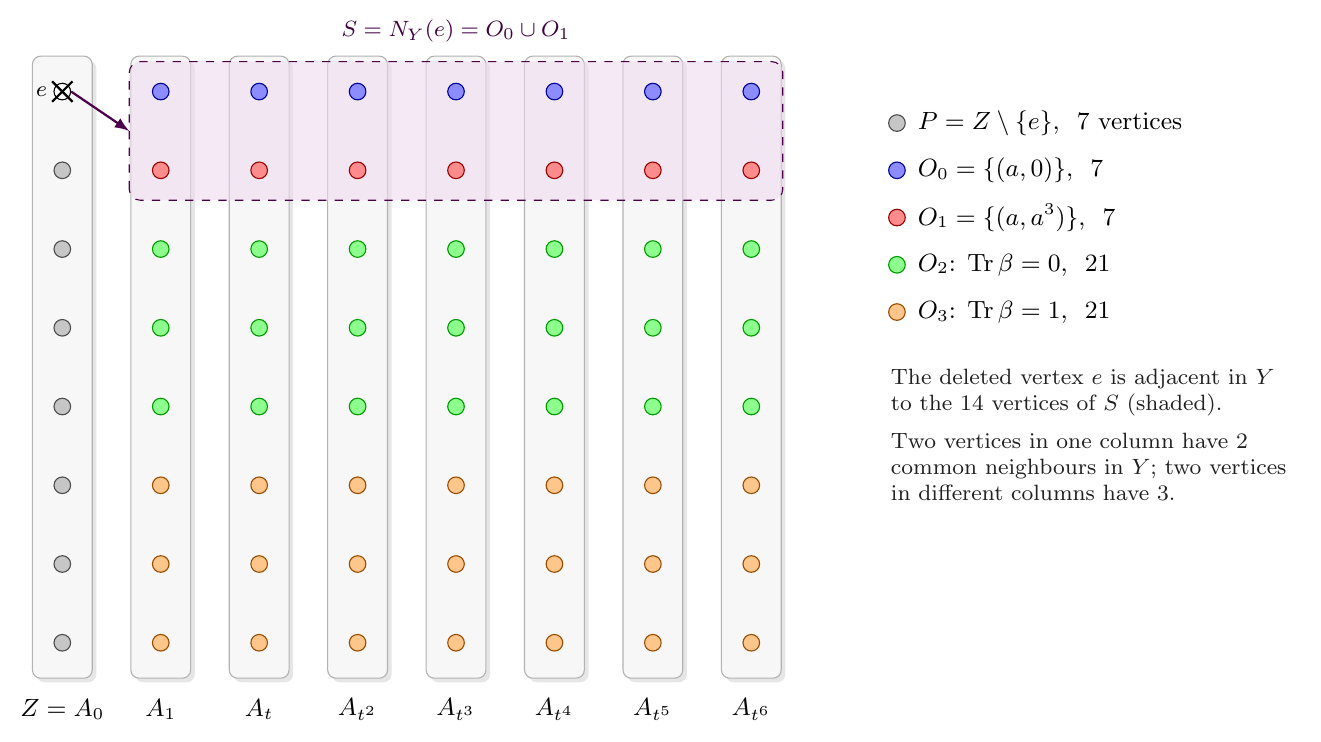
\includegraphics[width=\textwidth]{figures/fig_cosets.png}
\caption{The vertices of $Y$ arranged by the cosets of the centre $Z$. Deleting $e$ gives $X$; the fourteen neighbours of $e$ form $S=O_0\cup O_1$ and have degree $13$ in $X$. Each coset other than $Z$ meets $O_0$ and $O_1$ once and $O_2$ and $O_3$ three times.}\label{fig:cosets}
\end{figure}

\begin{lemma}\label{lem:K}
The group $K$ generated by the maps $\mu_c$ and $\varphi$ acts on each of $P,O_0,O_1,O_2,O_3$ transitively.
\end{lemma}

\begin{proof}
$\mu_c(0,b)=(0,c^3b)$, and cubing is onto $\F^\times$. Further $\mu_c(a,a^3\beta)=(ca,(ca)^3\beta)$ and $\varphi(a,a^3\beta)=(a^2,(a^2)^3\beta^2)$, while $\{\beta,\beta^2,\beta^4\}$ equals $R_0$ for $\beta\in R_0$ and $R_1$ for $\beta\in R_1$.
\end{proof}

\begin{lemma}\label{lem:extend}
Every automorphism of $X$ extends to an automorphism of $Y$ fixing $e$ and preserving each of the sets $P$, $S$ and $O_2\cup O_3$. Every automorphism of $Y$ permutes the cosets of $Z$.
\end{lemma}

\begin{proof}
In $X$ the vertices of $S=N_Y(e)$ have degree $13$ and all others degree $14$. So an automorphism $\sigma$ of $X$ maps $S$ onto $S$, and setting $\sigma(e)=e$ gives an automorphism of $Y$. By Lemma~\ref{lem:lambda} the cosets of $Z$ are the classes of the relation ``$g=h$, or $g$ and $h$ have exactly two common neighbours'', so every automorphism of $Y$ permutes them; one fixing $e$ maps $Z$ onto $Z$, hence $P=Z\setminus\{e\}$ onto $P$, and it maps the complement $O_2\cup O_3$ of $\{e\}\cup P\cup S$ onto itself.
\end{proof}

\begin{lemma}\label{lem:tau}
Let $a\ne c$. Each $u=(a,b)\in A_a$ has exactly two neighbours in $A_c$, namely $(c,b+a(a+c)^2)$ and $(c,b+c(a+c)^2)$, and $uz_{a+c}=(a,b+(a+c)^3)$ is the only other vertex of $A_a$ with the same two neighbours in $A_c$.
\end{lemma}

\begin{proof}
The neighbours come from Lemma~\ref{lem:adj}. The two values $\alpha=a(a+c)^2$ and $\alpha'=c(a+c)^2$ are distinct with $\alpha+\alpha'=(a+c)^3$. The vertex $(a,b')$ has the neighbour set $\{(c,b'+\alpha),(c,b'+\alpha')\}$, which equals that of $u$ if and only if $b'\in\{b,\ b+\alpha+\alpha'\}$.
\end{proof}

For distinct cosets $A,C$ let $\tau_{A,C}\colon A\to A$ map $u$ to the other vertex of $A$ with the same neighbours in $C$. By Lemma~\ref{lem:tau}, $\tau_{A_a,A_c}(u)=uz_{a+c}$, and $\sigma\tau_{A,C}\sigma^{-1}=\tau_{\sigma(A),\sigma(C)}$ for every automorphism $\sigma$ of $Y$, since the definition uses only adjacency and the coset partition. On $Z=A_0$ write $\tau_c=\tau_{Z,A_c}$, so $\tau_c(0,b)=(0,b+c^3)$. Call three distinct cosets $A_{c_1},A_{c_2},A_{c_3}\ne Z$ \emph{aligned} if $\tau_{c_1}\tau_{c_2}\tau_{c_3}$ is the identity of $Z$, that is, if $c_1^3+c_2^3+c_3^3=0$. An automorphism of $Y$ fixing $e$ fixes $Z$, conjugates $\tau_c$ to the map $\tau$ attached to $\sigma(A_c)$, and so maps aligned triples to aligned triples.

\begin{lemma}\label{lem:S}
Each $s\in S$ has exactly three neighbours in $S$, lying in three distinct cosets of $Z$. These cosets are aligned if $s\in O_0$ and not aligned if $s\in O_1$.
\end{lemma}

\begin{proof}
Let $s=(a,0)$ and $(c,d)\in S$ with $c\ne a$. For $d=0$, Lemma~\ref{lem:adj} would need $0\in\{a(a+c)^2,c(a+c)^2\}$, which is impossible. For $d=c^3$ it needs $c^3=c(a+c)^2$, which gives $a=0$, or $c^3=a(a+c)^2$, which for $x=c/a$ reads $x^3=x^2+1$, that is $x\in R_1$. So the neighbours of $s$ in $S$ are $(ax,(ax)^3)$, $x\in R_1$, in the cosets $A_{ax}$, and
\[
\sum_{x\in R_1}(ax)^3=a^3\sum_{x\in R_1}(x^2+1)=a^3\Bigl(\bigl(\textstyle\sum_{x\in R_1}x\bigr)^2+1\Bigr)=0 .
\]

Let $s=(a,a^3)$. For $(c,0)$ the condition is $a^3\in\{a(a+c)^2,c(a+c)^2\}$; the first gives $c=0$, the second, with $x=c/a$, gives $x^3+x=1$, that is $x\in R_0$. For $(c,c^3)$ it is $a^3+c^3\in\{a^3+ac^2,\ a^2c+c^3\}$, which gives $c=a$ in both cases. So the neighbours of $s$ in $S$ are $(ay,0)$, $y\in R_0$, in the cosets $A_{ay}$, and $\sum_{y\in R_0}(ay)^3=a^3\sum_{y\in R_0}(y+1)=a^3\ne0$.
\end{proof}

The aligned triples are the lines of a Fano plane on the seven cosets $A_c\ne Z$, since $c\mapsto c^3$ is a bijection of $\F^\times$ and the triples $\{x,y,x+y\}$ of nonzero elements of $\F$ are the lines of the Fano plane of the $\F_2$-space $\F$. Figure~\ref{fig:fano} shows this plane and Lemma~\ref{lem:S} for $a=1$.

\begin{figure}[ht]
\centering
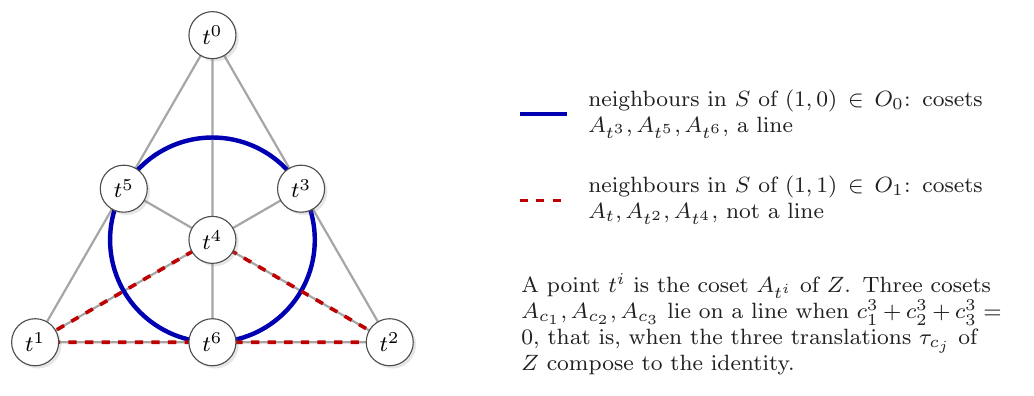
\includegraphics[width=\textwidth]{figures/fig_fano.png}
\caption{The seven cosets $A_c\ne Z$, $c=t^i$, as the points of a Fano plane whose lines are the aligned triples. The neighbours in $S$ of $(1,0)\in O_0$ lie in the cosets of a line, those of $(1,1)\in O_1$ do not.}\label{fig:fano}
\end{figure}

\begin{lemma}\label{lem:O23}
Each vertex of $O_2$ has one neighbour in $O_0$ and two in $O_1$; each vertex of $O_3$ has two neighbours in $O_0$ and one in $O_1$.
\end{lemma}

\begin{proof}
Let $v=(a,a^3\beta)$ with $\beta\in R_0\cup R_1$, and write a vertex of $S$ in a coset $A_c$, $c\notin\{0,a\}$, with $x=c/a\in\F^\circ$. Dividing the condition of Lemma~\ref{lem:adj} by $a^3$, the vertex $(c,0)$ is a neighbour of $v$ if and only if $\beta\in\{(1+x)^2,\ x+x^3\}$, and $(c,c^3)$ is a neighbour if and only if $\beta\in\{1+x^2+x^3,\ x\}$. In each pair the two values differ for $x\ne1$, so the number of neighbours of $v$ in $O_0$ is the number of solutions $x\in\F^\circ$ of $(1+x)^2=\beta$ plus that of $x+x^3=\beta$, and similarly for $O_1$.

The equations $(1+x)^2=\beta$ and $x=\beta$ have one solution each in $\F^\circ$. By the proof of Lemma~\ref{lem:lambda}, $x+x^3$ equals $1$ on $R_0$ and $x^4$ on $R_1$, and $1+x^2+x^3$ equals $x^4$ on $R_0$ and $0$ on $R_1$. So $x+x^3=\beta$ has one solution for $\beta\in R_1$ and none for $\beta\in R_0$, and $1+x^2+x^3=\beta$ has one solution for $\beta\in R_0$ and none for $\beta\in R_1$.
\end{proof}

\begin{theorem}\label{thm:orbits}
The orbits of $\Aut(X)$ on $V(X)$ are $P$, $O_0$, $O_1$, $O_2$, $O_3$. In particular $r(X)=5$.
\end{theorem}

\begin{proof}
By Lemmas~\ref{lem:aut} and~\ref{lem:K} each of the five sets lies in one orbit. Let $\sigma\in\Aut(X)$, extended to $Y$ by Lemma~\ref{lem:extend}. Then $\sigma$ preserves $P$ and $S$, permutes the cosets of $Z$, and maps aligned triples to aligned triples; as $\sigma$ permutes the finite set of triples, it also maps triples that are not aligned to triples that are not aligned. It maps the three neighbours in $S$ of a vertex $s\in S$ onto those of $\sigma(s)$, and their cosets onto the corresponding cosets. By Lemma~\ref{lem:S}, $\sigma(O_0)=O_0$ and $\sigma(O_1)=O_1$. Then $\sigma$ preserves $O_2\cup O_3$ and the numbers of neighbours in $O_0$ and in $O_1$, so $\sigma(O_2)=O_2$ and $\sigma(O_3)=O_3$ by Lemma~\ref{lem:O23}.
\end{proof}

\begin{remark}
A complete computer search for automorphisms shows that $Y$ has $1344=64\cdot21$ automorphisms and $X$ has $21$, so $\Aut(X)=K$. This is not used in the proof.
\end{remark}

\section{The cards}\label{sec:cards}

\begin{lemma}\label{lem:inverse}
For every vertex $x$ of $X$, the cards $X-x$ and $X-x^{-1}$ are isomorphic.
\end{lemma}

\begin{proof}
Left multiplication $g\mapsto x^{-1}g$ is an automorphism of $Y$ mapping $x$ to $e$ and $e$ to $x^{-1}$. It maps $V(Y)\setminus\{e,x\}$ onto $V(Y)\setminus\{e,x^{-1}\}$, so it restricts to an isomorphism $X-x=Y-\{e,x\}\to Y-\{e,x^{-1}\}=X-x^{-1}$.
\end{proof}

Inversion fixes $P$ pointwise, maps $(a,0)$ to $(a,a^3)$, and maps $(a,a^3\beta)$ to $(a,a^3(\beta+1))$ with $\Tr(\beta+1)=\Tr(\beta)+1$. So it exchanges $O_0$ with $O_1$ and $O_2$ with $O_3$. In particular each $x\in O_0\cup O_2$ is pseudosimilar to $x^{-1}$.

\begin{theorem}\label{thm:cards}
The cards of $X$ fall into exactly three isomorphism classes: those at the vertices of $P$, of $O_0\cup O_1$, and of $O_2\cup O_3$. In particular $k(X)=3$.
\end{theorem}

\begin{proof}
Cards at vertices in one orbit are isomorphic, so Theorem~\ref{thm:orbits} and Lemma~\ref{lem:inverse} give at most these three classes. To separate them, count the vertices of degree $13$ in $X-x=Y-\{e,x\}$. A vertex $u\ne e,x$ has degree $14-[u\sim e]-[u\sim x]$ there, so these vertices are those of the symmetric difference of $N_Y(e)$ and $N_Y(x)$ other than $e$ and $x$. Their number is $28-2\lambda(x)-2[x\in S]$, which by Lemma~\ref{lem:lambda} is $24$ for $x\in P$, $20$ for $x\in S=O_0\cup O_1$, and $22$ for $x\in O_2\cup O_3$.
\end{proof}

Theorem~\ref{thm:main} follows from Corollary~\ref{cor:conn} and Theorems~\ref{thm:orbits} and~\ref{thm:cards}. Figure~\ref{fig:cards} summarizes the argument.

\begin{figure}[ht]
\centering
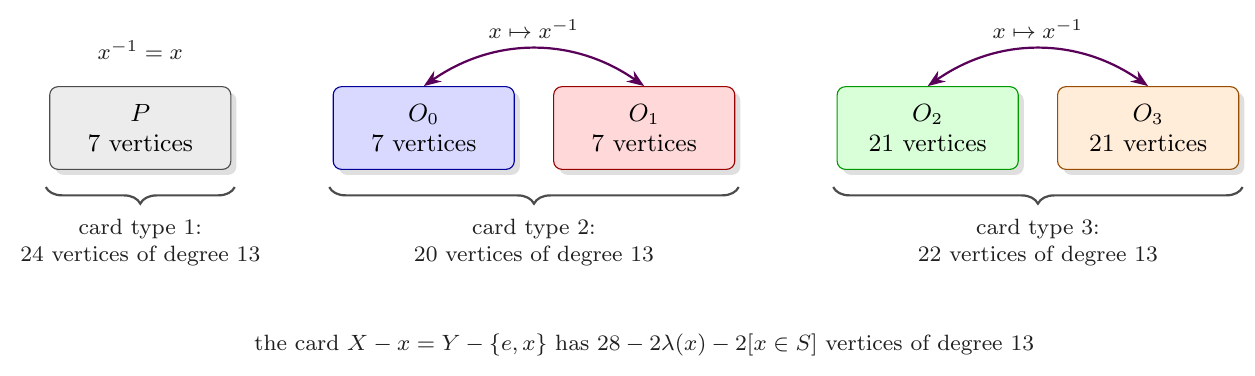
\includegraphics[width=\textwidth]{figures/fig_cards.png}
\caption{The five orbits of $\Aut(X)$ and the three card types. Inversion in $H$ fixes $P$ pointwise and exchanges $O_0$ with $O_1$ and $O_2$ with $O_3$, which gives the isomorphisms of Lemma~\ref{lem:inverse}; the number of vertices of degree $13$ separates the three types.}\label{fig:cards}
\end{figure}

\section{Formal verification and computations}\label{sec:lean}

Theorem~\ref{thm:main} is formalized in Lean~4 \cite{MU21} with Mathlib \cite{Mathlib20}, version~4.34.1, and the formal proof is checked by the Lean kernel. The formal statement says that there are a finite set $V$ with $63$ elements and a simple graph $G$ on $V$ such that $G$ is connected, the relation ``$G-v$ and $G-w$ are isomorphic'' on $V$ has exactly three classes, and the relation ``some automorphism of $G$ maps $v$ to $w$'' has exactly five classes. In the formal model the elements of $\F$ are coded by the integers $0,\dots,7$ through their coordinates in the basis $1,t,t^2$, the vertex $k\in\{0,\dots,62\}$ is the pair $(a,b)$ with $8a+b=k+1$, and adjacency is the formula of Lemma~\ref{lem:adj}. The proof depends only on the axioms of Lean's logic, namely propositional extensionality, choice and the soundness of quotients; it has no unproved step and adds no axiom.

The formal proof follows Sections~\ref{sec:graph}--\ref{sec:cards} with one change of route. It gives the automorphisms $\mu_t$ and $\varphi$ and the isomorphisms of Lemma~\ref{lem:inverse} explicitly, and separates the five orbits by a single invariant in place of the Fano plane: for a vertex $x$, the number of pairs $(y,z)$ with $x\sim y\sim z$, $z\ne x$, $z\not\sim x$, such that $x$ and $z$ have exactly two common neighbours and $y$ and $z$ have no common neighbour of degree $13$. Every automorphism preserves this number, and it takes the values $6,15,21,8,4$ on $P,O_0,O_1,O_2,O_3$. The finitely many instances of each lemma are evaluated by the kernel itself.

Independent computations in exact integer arithmetic confirm that $X$ has $63$ vertices and $434$ edges and is connected, that $\mu_t$ and $\varphi$ are automorphisms with the orbits of Lemma~\ref{lem:K}, the values of the invariant above, Lemma~\ref{lem:inverse} for every vertex, and the counts in the proof of Theorem~\ref{thm:cards}.

\section*{Declaration of generative AI and AI-assisted technologies in the manuscript preparation process}
During the preparation of this work the authors used Claude (Anthropic) in order to assist with the construction, the proofs, the Lean formalization, the computations and the preparation of the manuscript. After using this tool, the authors reviewed and edited the content as needed and take full responsibility for the content of the published article.

\section*{Data availability}
\begingroup\raggedright
Deep Bhattacharjee computed the Lean formalization and the Julia, C, C++, shell and Python computations with the help of AI assistance (Claude, Anthropic). The Lean formalization of the proofs in this paper is archived at Zenodo, doi:\href{https://doi.org/\zenodoID}{\zenodoID}. The paper is available at \url{\preprintURL}.\par
\endgroup

\section*{Competing interests}
None.

\section*{Funding}
None.

\bibliographystyle{elsarticle-num}
\bibliography{refs}

\end{document}
